\section{Data Curation, Evaluation Protocols, and Complete Depth Results}
\label{app:bonn-results}

Following the organization of the UniSH supplementary material, we first state the data and filtering boundaries before presenting the complete evaluation. This work uses the public 3DPW, EMDB, TUM-Dynamic, and Bonn datasets for their corresponding tasks; v0.3 does not claim to construct a new training dataset or a new collection of web videos. The final version must report the exact splits, number of valid samples, crop and resize operations, human-visibility rules, invalid-depth masks, and dataset licenses. Any filtering threshold that has not yet been verified remains explicitly marked as pending.

Table~\ref{tab:bonn-depth} is the original Table 3 moved from the main paper to the appendix. Our result is computed from the human-scale-calibrated model output without using GT scale or shift at test time. The red curves in Fig.~\ref{fig:general-reconstruction}, which fit a scale from GT, are oracle diagnostics only and are not predictions of our method. The remaining appendices document coordinate conventions, model architecture, training configuration, component impact, robustness, efficiency, and failure analysis.

\begin{table}[H]
\caption{Human-centered video depth estimation on Bonn. Lower Abs Rel and higher $\delta<1.25$ are better.}
\label{tab:bonn-depth}
\centering
\begin{tabular}{lcc}
\toprule
Method & Abs Rel $\downarrow$ & $\delta<1.25$ $\uparrow$ \\
\midrule
DUSt3R & 0.151 & 0.839 \\
MASt3R & 0.188 & 0.765 \\
MonST3R & 0.072 & 0.957 \\
Fast3R & 0.194 & 0.772 \\
MVDUSt3R & 0.426 & 0.357 \\
CUT3R & 0.078 & 0.937 \\
Aether & 0.273 & 0.594 \\
FLARE & 0.152 & 0.790 \\
VGGT & 0.057 & 0.966 \\
$\pi^3$ & 0.049 & 0.975 \\
Human3R & 0.086 & 0.954 \\
UniSH & \textbf{0.035} & \textbf{0.980} \\
\textbf{Ours} & 0.08599 & 0.96377 \\
\bottomrule
\end{tabular}
\end{table}

\section{Notation, Coordinate Systems, and Metric Gauge}
\label{app:coordinates}

This appendix provides implementation and evaluation details omitted from the main paper for clarity. Appendix~\ref{app:coordinates} specifies coordinate and scale conventions; Appendix~\ref{app:architecture} gives the complete inference procedure; Appendix~\ref{app:training} summarizes the training objectives; Appendix~\ref{app:evaluation} describes datasets and evaluation protocols; Appendices~\ref{app:ablation}--\ref{app:efficiency} reserve the real ablation, robustness, and efficiency results; and Appendix~\ref{app:limitations} records failure modes and responsible-use boundaries. Every red ``To be evaluated'' entry is an explicit placeholder and does not constitute a result or supporting evidence.

\subsection{Coordinate and Depth Conventions}

For frame $t$ and person $n$ in a clip, VGGT-Ω predicts relative scene depth and camera parameters, while NLF provides SMPL human observations expressed in meters. We establish correspondences between human surfaces and scene depth using Z-depth along the camera optical axis; Euclidean distance along a camera ray is not treated as Z-depth. Camera coordinates, world coordinates, camera-to-world transformations, and matrix multiplication follow the conventions of Eqs.~\ref{eq:metric-depth-overview}--\ref{eq:translation-overview}.

Let $D^{\mathrm{rel}}$ denote relative depth, $s_{\mathrm{clip}}$ the shared clip-level scale, and $b_{\mathrm{clip}}$ the residual depth bias. Metric depth and metric camera translation are
\begin{equation}
D^{\mathrm{metric}} = s_{\mathrm{clip}}D^{\mathrm{rel}} + b_{\mathrm{clip}},
\qquad
\mathbf{t}^{\mathrm{metric}} = s_{\mathrm{clip}}\mathbf{t}^{\mathrm{rel}}.
\label{eq:appendix-metric-propagation}
\end{equation}
The bias acts only in the depth domain and is not directly added to camera translation. After shared-scale propagation, TRSTR performs a constrained camera-space translation update on the human root, while pose and shape remain frozen.

\subsection{Tensor, Precision, and Device Conventions}

\begin{table}[H]
\caption{Main tensors and implementation conventions. Exact dimensions follow the final implementation configuration.}
\label{tab:tensor-conventions}
\centering
\small
\begin{tabular}{llll}
\toprule
Object & Main dimensions & Unit/coordinates & Status \\
\midrule
Input images & $B\times T\times3\times H\times W$ & image plane & defined \\
Relative depth & $B\times T\times H\times W$ & relative Z-depth & defined \\
SMPL vertices & $B\times T\times N\times V\times3$ & camera, meter & defined \\
Human anchors & $B\times T\times N\times24\times C$ & feature space & defined \\
TRSTR regions & $B\times T\times N\times96\times C_r$ & canonical body & defined \\
Exact dtype/device & -- & -- & \todoresult \\
\bottomrule
\end{tabular}
\end{table}

\section{Model Architecture Details and Complete Inference}
\label{app:architecture}

\subsection{VGGT-Ω, NLF, and Baseline Boundaries}

VGGT-Ω provides relative scene structure, camera parameters, and multi-level scene features. NLF provides local human pose, shape, camera-space translation, and confidence. GroundedHuman does not replace either baseline, and TRSTR is not allowed to reduce world-space error by changing pose or shape. The final version must list frozen parameters, trainable parameters, input resolution, clip length, and the maximum number of person slots.

\placeholdernote{The frozen-module inventory, checkpoint paths, input shapes, dtypes, devices, and memory configuration must be verified against the server implementation.}

\subsection{Visible-front-surface Analytic Scale}

For every valid person, the SMPL surface is projected into the relative-depth map, and a z-buffer-like front-surface test retains the visible body surface closest to the camera at shared pixels. Ratios between human Z-depth and relative scene Z-depth at valid pixels form scale proposals; a robust median removes the dominant scale freedom. In multi-person scenes, person-level proposals are aggregated into a clip-scale candidate according to visible support and confidence.

The final version must report the minimum number of valid pixels, depth-boundary exclusion radius, MAD or outlier threshold, ratio clamp, $\varepsilon$, low-confidence fallback, and handling of clips without a visible person.

\subsection{Person-conditioned Residual Affine}

Each person is represented by 24 canonical anchors. The module queries local depth residuals and multi-level VGGT-Ω scene features near the projected human, and outputs a near-identity residual scale and depth bias. Analytic geometry determines the scale magnitude; the learned module models only residual errors caused by occlusion, projection, and local depth bias.

\placeholdernote{Transformer/MLP depth, hidden dimension, attention heads, normalization, initialization, output range, and anchor fallback must be filled from the verified configuration.}

\subsection{Clip-level Consensus and Camera Propagation}

Frame- and person-level scales are first aggregated over valid people and then combined into a shared clip scale, which acts on both scene depth and camera translation. Frames with short-term human invisibility should reuse or smooth a reliable clip scale. The fallback for long intervals without a person must be explicitly specified; the latest valid scale must not be propagated indefinitely by default.

\subsection{Complete TRSTR Update}

TRSTR organizes the SMPL surface into 96 canonical body regions and separately samples self-surface, environment, and other-human geometry around each region. Every region predicts a bounded translation vote in a camera ray/tangent basis. A region gate, predicted uncertainty, and a person gate aggregate the regional votes into the human-root update. After each update, the human is reprojected and scene evidence is resampled, forming a two-step geometric loop.

\begin{equation}
\Delta\mathbf{t} = g_{\mathrm{person}}
\frac{\sum_r g_r\exp(-u_r)\Delta\mathbf{t}_r}
{\sum_r g_r\exp(-u_r)+\varepsilon},
\qquad
\mathbf{t}^{(k+1)}=\mathbf{t}^{(k)}+\operatorname{clip}(\Delta\mathbf{t},d_{\max}).
\label{eq:appendix-trstr-update}
\end{equation}

The final version must report the construction of the 96 regions, the number of vertices per region, probe radii, annulus definition, ray/tangent basis, gate heads, $d_{\max}$, and the stopping rule.

\begin{figure}[H]
\centering
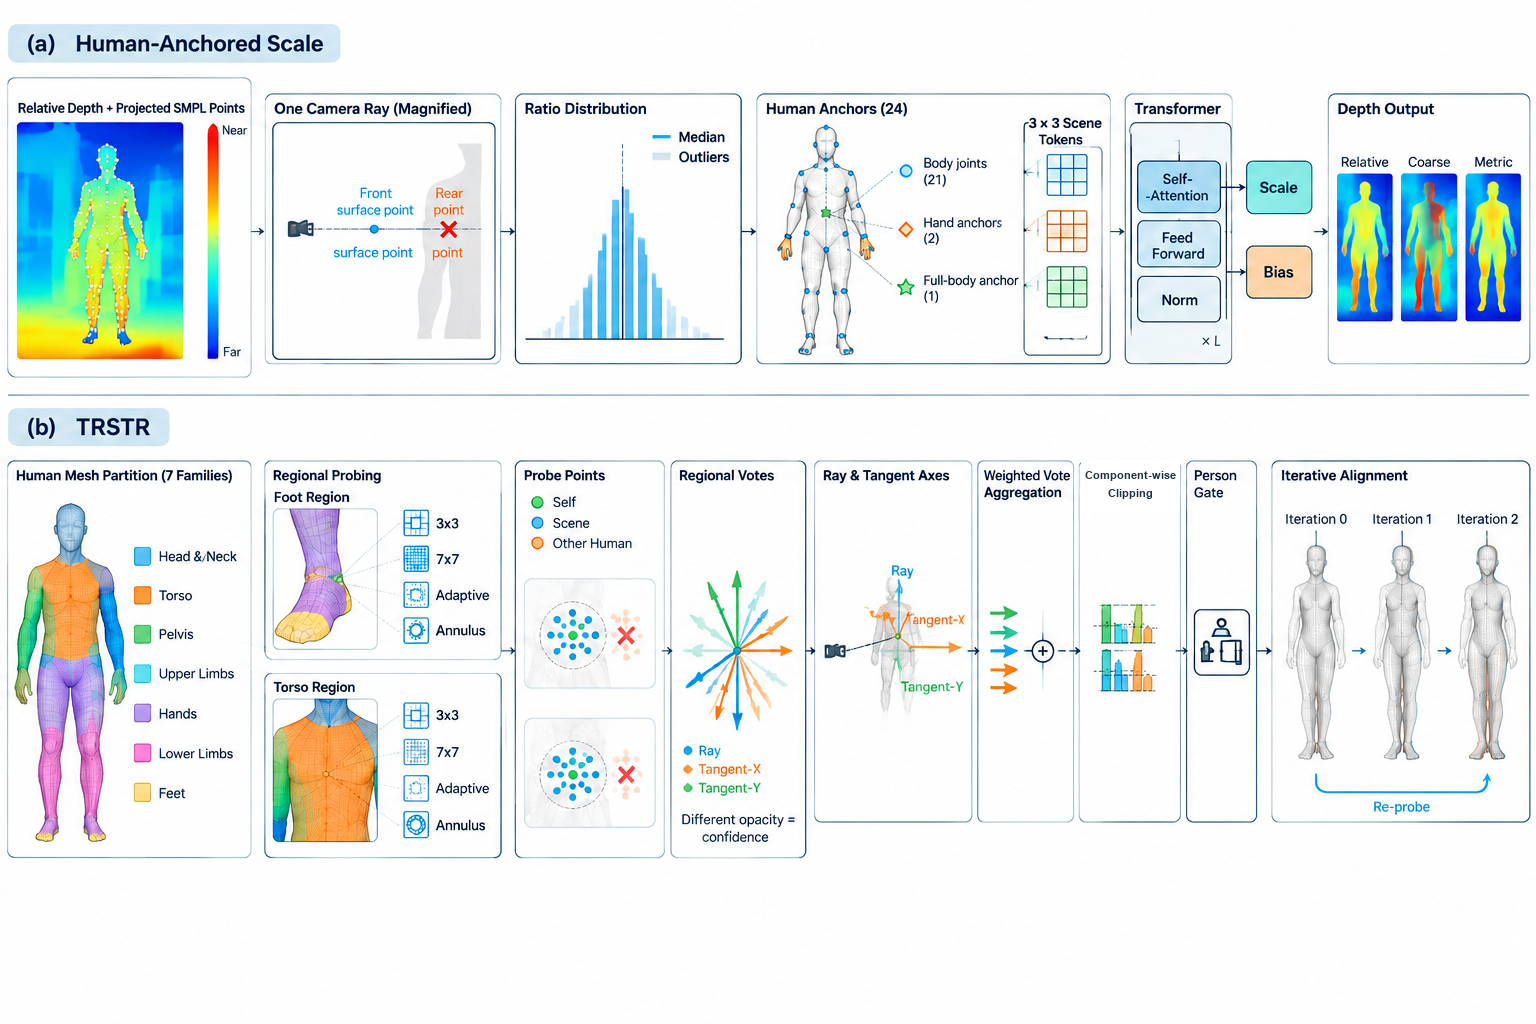
\includegraphics[width=\textwidth]{figures/fig3_scale_trstr_detail_final.png}
\caption{\textbf{Complete architecture of human-scale bridging and regional translation refinement.} (a) The human front surface projected into the relative-depth map provides an analytic coarse scale, and 24 HSI anchors use local scene features to predict residual scale and bias. (b) TRSTR partitions the human surface into deterministic regions and iteratively corrects translation using multi-scale human--environment probing, gating, and uncertainty-weighted regional votes while preserving pose and shape. This detail figure is moved from the main paper to the appendix.}
\label{fig:method-detail}
\end{figure}

\subsection{Inference Algorithm}

{\small
\begin{enumerate}
\setlength{\itemsep}{0pt}
\setlength{\parskip}{0pt}
\item Run the frozen VGGT-Ω to obtain relative depth, cameras, and scene features.
\item Run the frozen NLF to obtain local humans and confidence values.
\item Project the visible SMPL front surface and compute person/frame scale proposals.
\item Apply robust aggregation to obtain the analytic coarse scale.
\item Run the person-conditioned residual affine module to obtain residual scale and depth bias.
\item Aggregate the shared scale within the clip and propagate it to depth and camera translation.
\item Run two TRSTR iterations, updating only each person's root translation.
\item Output humans, scene geometry, and camera trajectories in a shared world coordinate system.
\end{enumerate}
}

\section{Implementation and Training Details}
\label{app:training}

\subsection{Staged Training}

The main paper uses two training stages: scale calibration and TRSTR. The scale stage must cover coarse residuals, depth bias, and perturbations of human visibility. The TRSTR stage must cover clean, scale-error, NLF-like, and mixed-error states, using staged remaining targets to supervise the residual translation after each iteration.

\begin{table}[H]
\caption{v0.3 training-configuration placeholders. Every red entry must be replaced with a verified server configuration.}
\label{tab:training-placeholder}
\centering
\small
\begin{tabular}{ll}
\toprule
Item & Configuration \\
\midrule
Training/validation split & \todoresult \\
Input resolution and clip length & \todoresult \\
Optimizer / learning rate & \todoresult \\
Scheduler / warm-up & \todoresult \\
Batch size / accumulation & \todoresult \\
Epochs or steps & \todoresult \\
Mixed precision / gradient clipping & \todoresult \\
GPU, training time, and random seed & \todoresult \\
Checkpoint selection & \todoresult \\
\bottomrule
\end{tabular}
\end{table}

\subsection{Complete Losses and Weights}

Equations~\ref{eq:scale-loss} and~\ref{eq:trstr-loss} define the two total objectives. The final version must provide the exact definitions and weights of the scale, bias, identity, vote, translation, gate, regularization, no-worse, and monotonic losses, and state whether the weights were selected through magnitude matching or sensitivity analysis on a held-out validation set.

\placeholdernote{Loss weights must not be filled with expected values; they must be extracted from training configurations and checkpoint records.}

\subsection{Training Stages and Freezing Strategy}

Following UniSH's practice of separating geometric objectives into consecutive training stages, the final GroundedHuman implementation description should report the scale-calibration stage and the TRSTR stage separately. During scale calibration, VGGT-Ω and NLF are frozen, and only the person-conditioned residual affine module and its output heads are trained. Training samples should cover correct initialization, coarse-scale residuals, depth bias, local occlusion, and changes in human visibility. During TRSTR training, the upstream scene and human backbones remain frozen, and the optimized variable is explicitly restricted to root translation so that pose and shape do not receive gradient updates.

Both stages must report the training and validation data sources, sampling ratios, frames per clip, number of people, perturbation ranges, and curriculum order. If a training variant fails to converge, the final paper should state ``non-convergent'' and define the diagnostic criterion, following UniSH's analysis of removing coarse alignment, rather than presenting an unsupported visualization. The checkpoint-selection metric and whether ablations share the same random seeds and data order must also be recorded.

\section{Complete Evaluation Protocols}
\label{app:evaluation}

\begin{table}[H]
\caption{Summary of tasks, datasets, and evaluation boundaries. Exact splits, sample counts, and preprocessing remain to be completed.}
\label{tab:evaluation-protocol}
\centering
\small
\resizebox{\textwidth}{!}{%
\begin{tabular}{lllll}
\toprule
Dataset & Task & Metrics & Alignment/GT use & Status \\
\midrule
3DPW & local human & PA-MPJPE, MPJPE, PVE & standard human protocol & partially known \\
EMDB-2 & world motion & WA-MPJPE, W-MPJPE, RTE & clips of at most 100 frames & partially known \\
TUM-Dynamic & camera trajectory & ATE & Sim(3) alignment & known \\
Bonn & metric video depth & Abs Rel, $\delta<1.25$ & no test-time GT scale/shift & known \\
Exact split/mask/averaging & -- & -- & -- & \todoresult \\
\bottomrule
\end{tabular}
}
\end{table}

\section{Impact of Human Metric Anchoring}
\label{app:ablation}

This section is intended to determine whether the gains arise from analytic scale, residual affine calibration, clip-level consensus, and TRSTR rather than from a naive combination of VGGT-Ω and NLF. v0.3 does not fabricate missing results. Table~\ref{tab:ablation-placeholder} and Fig.~\ref{fig:appendix-placeholder} define the structure to be populated by the final experiments.

\begin{table}[H]
\caption{Placeholder for cumulative component ablation. Every result requires a real experiment; this table supports no performance conclusion in its current form.}
\label{tab:ablation-placeholder}
\centering
\small
\resizebox{\textwidth}{!}{%
\begin{tabular}{lccccc@{\qquad}cccc}
\toprule
Variant & Analytic & Res. scale & Bias & Clip scale & TRSTR & W-MPJPE $\downarrow$ & RTE $\downarrow$ & Abs Rel $\downarrow$ & $\delta$ $\uparrow$ \\
\midrule
VGGT-Ω + NLF & & & & & & \todoresult & \todoresult & \todoresult & \todoresult \\
+ coarse scale & \cmark & & & & & \todoresult & \todoresult & \todoresult & \todoresult \\
+ residual scale & \cmark & \cmark & & & & \todoresult & \todoresult & \todoresult & \todoresult \\
+ depth bias & \cmark & \cmark & \cmark & & & \todoresult & \todoresult & \todoresult & \todoresult \\
+ clip consensus & \cmark & \cmark & \cmark & \cmark & & \todoresult & \todoresult & \todoresult & \todoresult \\
Full GroundedHuman & \cmark & \cmark & \cmark & \cmark & \cmark & \todoresult & \todoresult & \todoresult & \todoresult \\
\bottomrule
\end{tabular}
}
\end{table}

\begin{figure}[H]
\centering
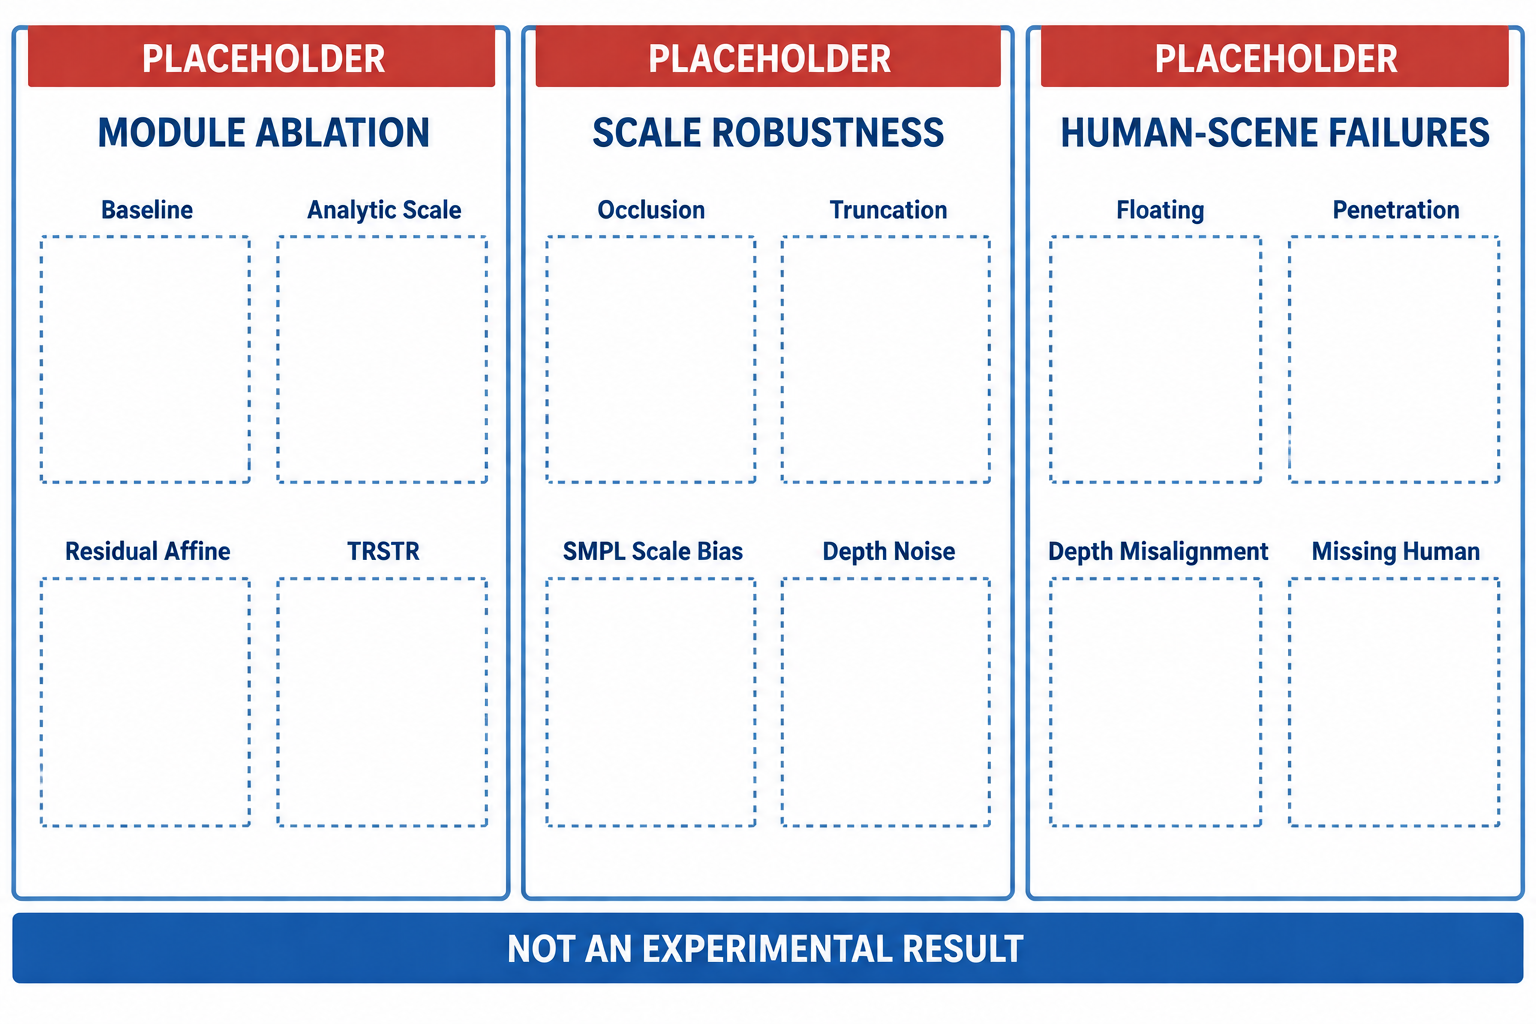
\includegraphics[width=0.96\textwidth]{figures/fig_appendix_placeholder_v2.png}
\caption{\textbf{Appendix experiment placeholder.} This NBAI-generated image previews the intended layout for ablation, robustness, and failure-case results. It is prominently marked as PLACEHOLDER and contains no real samples, values, or experimental conclusions. It must be completely replaced with verified server results in the final version.}
\label{fig:appendix-placeholder}
\end{figure}

The real ablation suite should compare visible front surfaces with root/joint anchors, median with mean aggregation, scale-only, bias-only, and scale-plus-bias calibration, frame-level with clip-level scale, single- with multi-person consensus, and the TRSTR region representation, ray/tangent voting, gates, uncertainty, person gate, and iteration count. It should also include zero-residual and shuffled-conditioning counterfactuals and a numerical pose/shape invariance check.

\section{TRSTR Refinement, Robustness, and Sensitivity}
\label{app:robustness}

\begin{table}[H]
\caption{Robustness experiment placeholder. The bins and perturbation ranges define the experimental design and do not represent completed results.}
\label{tab:robustness-placeholder}
\centering
\small
\resizebox{\textwidth}{!}{%
\begin{tabular}{lllcccc}
\toprule
Factor & Bin/perturbation & Main issue & W-MPJPE & RTE & Abs Rel & $\delta<1.25$ \\
\midrule
Visible human area & small/medium/large & anchor support & \todoresult & \todoresult & \todoresult & \todoresult \\
Occlusion/truncation & low/medium/high & front-surface validity & \todoresult & \todoresult & \todoresult & \todoresult \\
SMPL scale perturbation & $\pm5/10/15\%$ & metric-prior bias & \todoresult & \todoresult & \todoresult & \todoresult \\
Number of people & 1/2/$\geq3$ & multi-person consensus & \todoresult & \todoresult & \todoresult & \todoresult \\
Frames without a human & 0--100\% & scale fallback & \todoresult & \todoresult & \todoresult & \todoresult \\
Relative-depth noise & controlled perturbation & upstream propagation & \todoresult & \todoresult & \todoresult & \todoresult \\
\bottomrule
\end{tabular}
}
\end{table}

Errors in real human dimensions or SMPL shape directly affect absolute scale and are therefore the most important robustness risk for GroundedHuman. The final version must report this experiment; ordinary successful qualitative examples are not a substitute.

\section{Efficiency, Parameters, and Scalability}
\label{app:efficiency}

\begin{table}[H]
\caption{Placeholder for efficiency and resource usage. Test conditions and values require server measurements.}
\label{tab:efficiency-placeholder}
\centering
\small
\begin{tabular}{lccc}
\toprule
Module & Time & Peak memory & Parameters \\
\midrule
VGGT-Ω & \todoresult & \todoresult & frozen \\
NLF & \todoresult & \todoresult & frozen \\
Front-surface scale & \todoresult & \todoresult & 0 \\
HSI residual affine & \todoresult & \todoresult & \todoresult \\
TRSTR & \todoresult & \todoresult & \todoresult \\
End-to-end & \todoresult & \todoresult & \todoresult \\
\bottomrule
\end{tabular}
\end{table}

Final measurements must fix the GPU, input resolution, clip length, and number of people, and state whether data loading, human detection, visualization, and disk I/O are included. A quality--runtime trade-off for the number of TRSTR iterations should also be reported.

\section{Additional Qualitative Results, Failure Cases, and Responsible Use}
\label{app:limitations}

The contents corresponding to Figs.~\ref{fig:temporal-4d}, \ref{fig:general-reconstruction}, and~\ref{fig:metric-measurement} remain in the main paper to present temporal reconstruction, general 3D diagnostics, and interpretable real-world measurements. The final supplementary material should additionally show coarse scale, residual affine calibration, and TRSTR before/after results for the same sequences, together with cases involving occlusion, truncation, mutual occlusion among multiple people, long intervals without a visible human, and upstream depth failure.

The main failure chains include insufficient anchor support caused by invisibility or severe truncation; biased metric priors caused by incorrect SMPL shape or height; unreliable local probes caused by VGGT-Ω relative-structure errors; failed environment/other-human separation under dynamic objects or multi-person occlusion; and the inability of translation-only TRSTR to correct pose, shape, or fine-grained contact.

\placeholdernote{The final version must replace the FAILURE CASES panel in Fig.~\ref{fig:appendix-placeholder} with real failure samples and report detection signals, fallback behavior, and unresolved limitations.}

Human-video reconstruction may be misused for privacy-sensitive behavioral analysis or surveillance. This work is limited to geometric reconstruction and does not perform identity recognition or sensitive-attribute inference. Canonical human dimensions may also produce systematic scale bias for children, uncommon body types, or populations outside the training distribution; this issue must be quantified through the real sensitivity experiments in Appendix~\ref{app:robustness}.
